%%%%%%%%%%%%%%%%%%%%%%%%%%%%%%%%%%%%%%%%%%%%%%
%                insertmeeting
% 1) Title (something creative & funny?)
% 2) Date (MM/DD/YYYY)
% 3) Location (ex. Hagerty High School)
% 4) People/Committees Present 
% 5) Picture 
% 6) Start Time & Stop Time (ex. 12:30AM to 4:30PM)
%%%%%%%%%%%%%%%%%%%%%%%%%%%%%%%%%%%%%%%%%%%%%%
\insertmeeting 
	{Looking for Localization} 
	{01/10/22} 
	{Hagerty High School}
	{Annika, Anouska, Clayton, Falon, James, Jensen, Nathan, Ritam, Rose, Samantha, Lilly}
	{Images/RobotPics/robot.jpg}
	{2:30 - 4:30}
	
\hhscommittee{Software}
\noindent\hfil\rule{\textwidth}{.4pt}\hfil
\subsubsection*{Goals}
\begin{itemize}
    \item Attempt to derive equations for tricycle localization

\end{itemize} 

\noindent\hfil\rule{\textwidth}{.4pt}\hfil

\subsubsection*{Accomplishments}
Building onto the discoveries made in last week's meeting, we began to try to derive formulas that we can use in our tricycle drive. The most interesting resource we found today was a PowerPoint describing potential approaches to tricycle kinematics. As we read through the slides, we began to understand how we should approach the problem. Our measurements would come in a different format than typical 3 wheel odometry set ups, meaning we had to use new equations. Following the PowerPoint, we were able to successfully derive the necessary equations. 
 

\begin{figure}[ht]
\centering
\begin{minipage}[b]{.48\textwidth}
  \centering
  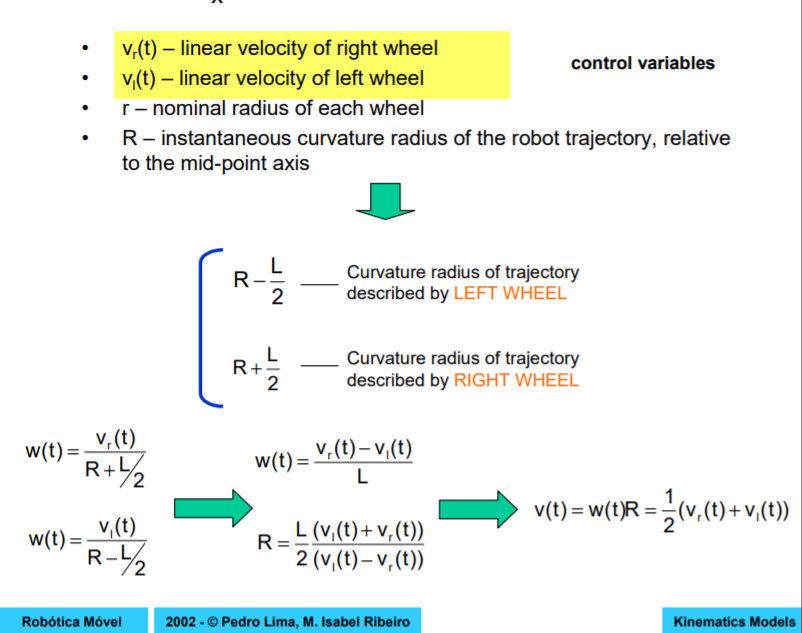
\includegraphics[width=0.95\textwidth]{Meetings/January/01-10-22/1.11.21 tricycle kinematics equations - James Hu.png}
  \caption{A slide from a lecture showing derivations of tricycle localization formulas}
  \label{fig:011022_1}
\end{minipage}%
\hfill%
\begin{minipage}[b]{.48\textwidth}
  \centering
  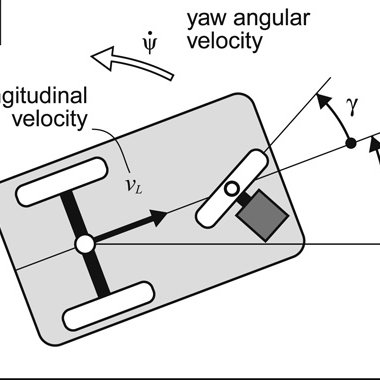
\includegraphics[width=0.95\textwidth]{Meetings/January/01-10-22/1.11.22 tricycle diagram - James Hu.jpg}
  \caption{Diagram of our drivetrain and variables needed}
  \label{fig:011022_2}
\end{minipage}
\end{figure}

\begin{figure}[htp]
\centering
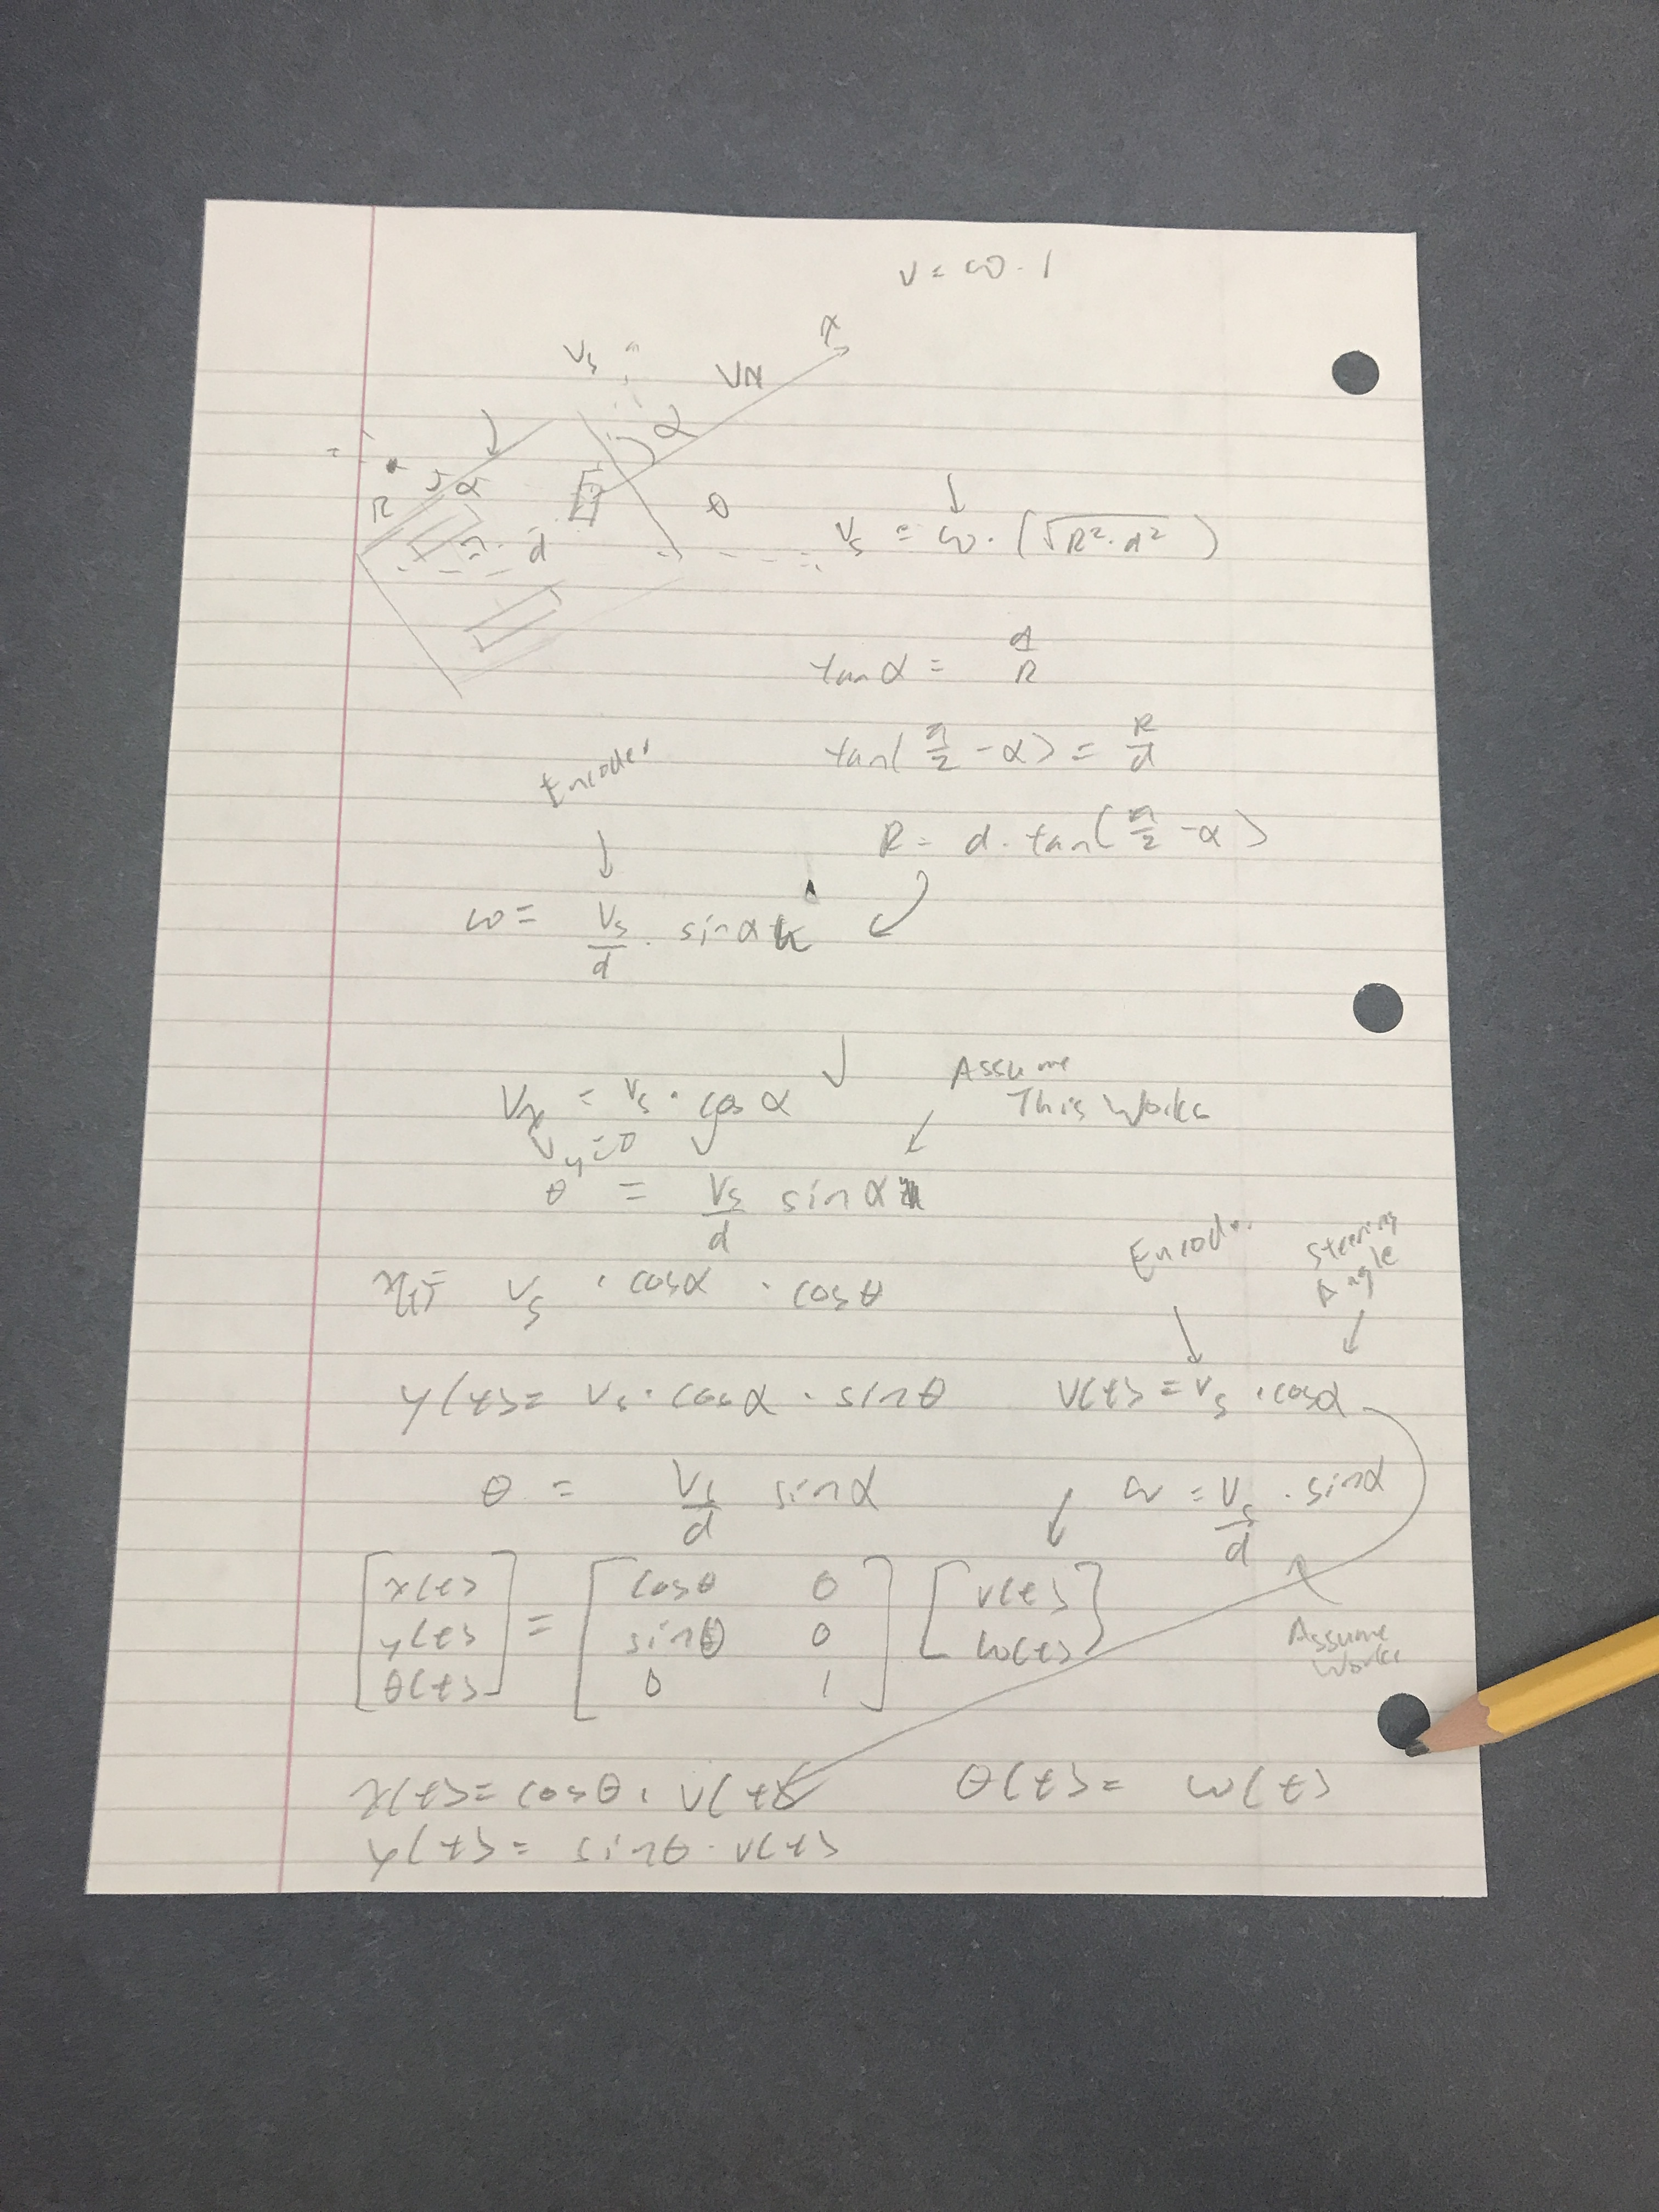
\includegraphics[width=0.95\textwidth, angle=0]{Meetings/January/01-10-22/1.11.22 paper derivation - James Hu.JPG}
\caption{Our derivation of formulas for change in x and change in heading to use in our robot}
\label{fig:011022_3}
\end{figure}

\whatsnext{
\begin{itemize}
    \item Implement the derived equations in Java
\end{itemize} 
}

